\pagestyle{empty}
\cleardoublepage
\pagestyle{fancy}

\chapter{Geração de Malhas}\label{cap3}

Nesse capítulo, serão apresentadas técnicas de geração de malhas bidimensionais, algumas sequenciais, outras em paralelo. As técnicas aqui discutidas enquadram-se em três categorias:

\begin{itemize}
  \item Avanço de fronteira, onde a malha deve ser criada a partir da entrada que forma o contorno da região;

  \item Delaunay, onde tenta-se maximizar o menor ângulo dos triângulos gerados para um dado conjunto de pontos;

  \item Arbitrária, que são os outros tipos de malhas;
\end{itemize}

\section{Avanço de fronteira}

Os algoritmos de avanço de fronteira partem de um contorno especificado da região a ser preenchida (fig.~\ref{fig:imagem7}a). Este contorno é chamado de fronteira inicial ou borda, os elementos são gerados por vez a partir dessa fronteira. A medida que os polígonos são gerados, a fronteira é atualizada, sempre removendo ou adicionando elementos de fronteira. O algoritmo termina quando não há mais fronteira, indicando que a região foi totalmente preenchida, ou quando não é possível gerar mais nenhum elemento mesmo com fronteira, indicando que o algoritmo falhou.

Uma fronteira bidimensional é formada por um conjunto de arestas. Essa técnica geralmente faz uso de pontos de Steiner, ou seja, insere novos pontos, que não pertencem à entrada, esse pontos criados irão pertencer aos elementos gerados. Um algoritmo nessa categoria procede da seguinte forma, no caso 2D triangular (fig.~\ref{fig:imagem7}b), enquanto houver arestas na fronteira:
 
 \begin{enumerate}
\item{ Remova uma aresta da fronteira, a aresta base (fig.~\ref{fig:imagem7}b)}
\item{ Encontre um ponto ideal para a formação de um novo triângulo com a aresta base (fig.~\ref{fig:imagem7}c),}
\item{ Crie uma região de busca em torno desse ponto ideal (fig.~\ref{fig:imagem7}d),}
\item{ Selecione o ponto dentro dessa região de busca cujo triângulo (entre esse ponto e a aresta base) seja válido e seja o de melhor qualidade,}
\item{ Forme o novo triângulo com o ponto selecionado e adicione-o à malha (fig.~\ref{fig:imagem7}e),}
\item{ Atualize a fronteira, inserindo as arestas que foram criadas, e removendo as arestas que já existiam,}
\item{ Se existir aresta na fronteira, volte para o passo 1.}
\end{enumerate}

 \begin{figure}[htbp]
     \centering
     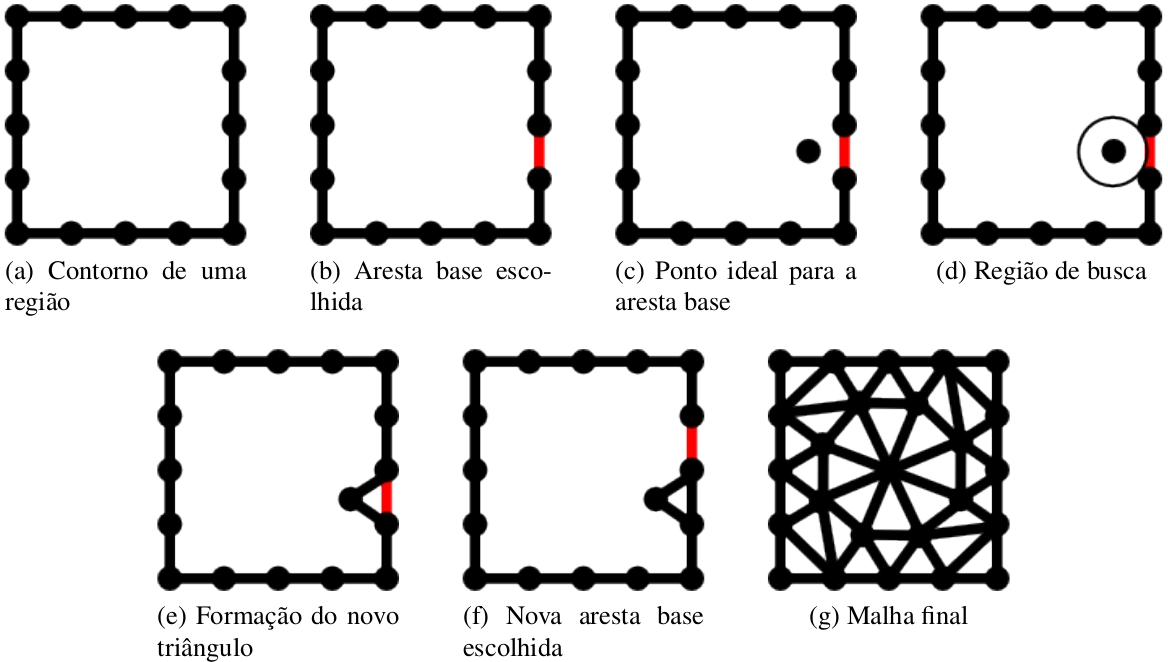
\includegraphics[width=1\textwidth]{imagem7}
     \caption{Avanço de fronteira.}
     \label{fig:imagem7}
 \end{figure}

Os algoritmos de avanço de fronteira têm facilidade em tratar regiões descontínuas, ou por conterem buracos, ou por serem regiões separadas, uma vez que a fronteira é sempre respeitada. Além disso, os elementos próximos à fronteira são, geralmente, de boa qualidade, provendo estabilidade e precisão na aplicação de métodos numéricos (como os métodos dos elementos finitos) sobre a malha gerada.

Entretanto, em alguns casos os elementos mais internos à malha nem sempre são de boa qualidade, pois a região torna-se menor a medida que a fronteira avança. Para tratar esses casos, geralmente uma técnica de suavização ou otimização é aplicada na malha resultante do algoritmo. Existem, ainda, alguns casos onde o algoritmo falha em gerar a malha, geralmente em casos tridimensionais.




